\section{Segmentação Textual}


% -- Definição da Tarefa e de Segmentação
A tarefa de segmentação textual consiste em dividir um texto em partes ou segmentos que contenham um significado relativamente independente. Em outras palavras, é identificar as posições nas quais há uma mudança significativa de assuntos. As técnicas de segmentação textual consideram um texto como uma sequência linear de unidades de informação que podem ser, por exemplo, cada termo presente no texto, os parágrafos ou as sentenças. Cada unidade de informação é um elemento do texto que não será dividido no processo de segmentação e cada ponto entre duas unidades é considerado um candidato a limite entre segmentos. Nesse sentido, um segmento pode ser visto como uma sucessão de unidades de informação que compartilham o mesmo assunto.




% -- Algoritmos

\subsection{Algoritmos de Segmentação Textual}
% ==========  Janelas deslizantes  ==========


%  Coesão léxica como presuposto básico
Os primeiros trabalhos dessa área se apoiam na ideia de que a mudança de assunto em um texto é acompanhada de uma proporcional mudança de vocabulário. Essa ideia, chamada de coesão léxica, sugere que a distribuição das palavras é um forte indicador da estrutura do texto, e demonstrou-se que há uma estreita correlação entre quedas na coesão léxica em janelas de texto e a transição de assuntos~\cite{Kozima1993}. Em seu trabalho, Kozima calculou a coesão léxica de uma janela de palavras usando \textit{spreading activation} em uma rede semântica especialmente elaborada para o idioma Inglês. Contudo, a implementação de um algoritmo para outros domínios depende da construção de uma rede adequada. 



O conceito de coesão léxica permite a aplicação da técnica de janelas deslizantes para encontrar os segmentos de um texto, em que se verifica a frequência dos termos em um fragmento do documento. Inicialmente, estabelece-se a partir do início do texto, um intervalo de $t$ termos, chamado janela que em seguida é deslocada em passos de $k$ termos adiante até o final do texto. A cada passo, analisa-se os termos contidos na janela.



% ==========  TextTiling  ==========

% Rafael --> Podem ter vários tipos de cursa. Ser mais objetivo. Quando a similaridade fica abaixo de um limiar fornecido pelo usuário.? Na verdade, dá pra fazer uma mescla. 

O conceito de coesão léxica motivou a elaboração dos primeiros algoritmos para segmentação textual, entre eles o \textit{TextTiling}. O \textit{TextTiling} baseia-se na ideia de que um segmento pode ser identificado pela análise dos termos que o compõe. Inicialmente, o \textit{TextTiling} recebe uma lista de candidatos a limite entre segmentos, usualmente finais de parágrafo ou finais de sentença. Utilizando a técnica de janelas deslizantes, para cada posição candidata são construídos 2 blocos, um contendo as sentenças que a precedem e outro com as que a sucedem. O tamanho desses blocos é um parâmetro a ser fornecido ao algoritmo e determina o tamanho mínimo de um segmento. Esse processo é ilustrado na Figura~\ref{fig:TT-slidingwindow}.



\begin{figure}[h!]
\center
	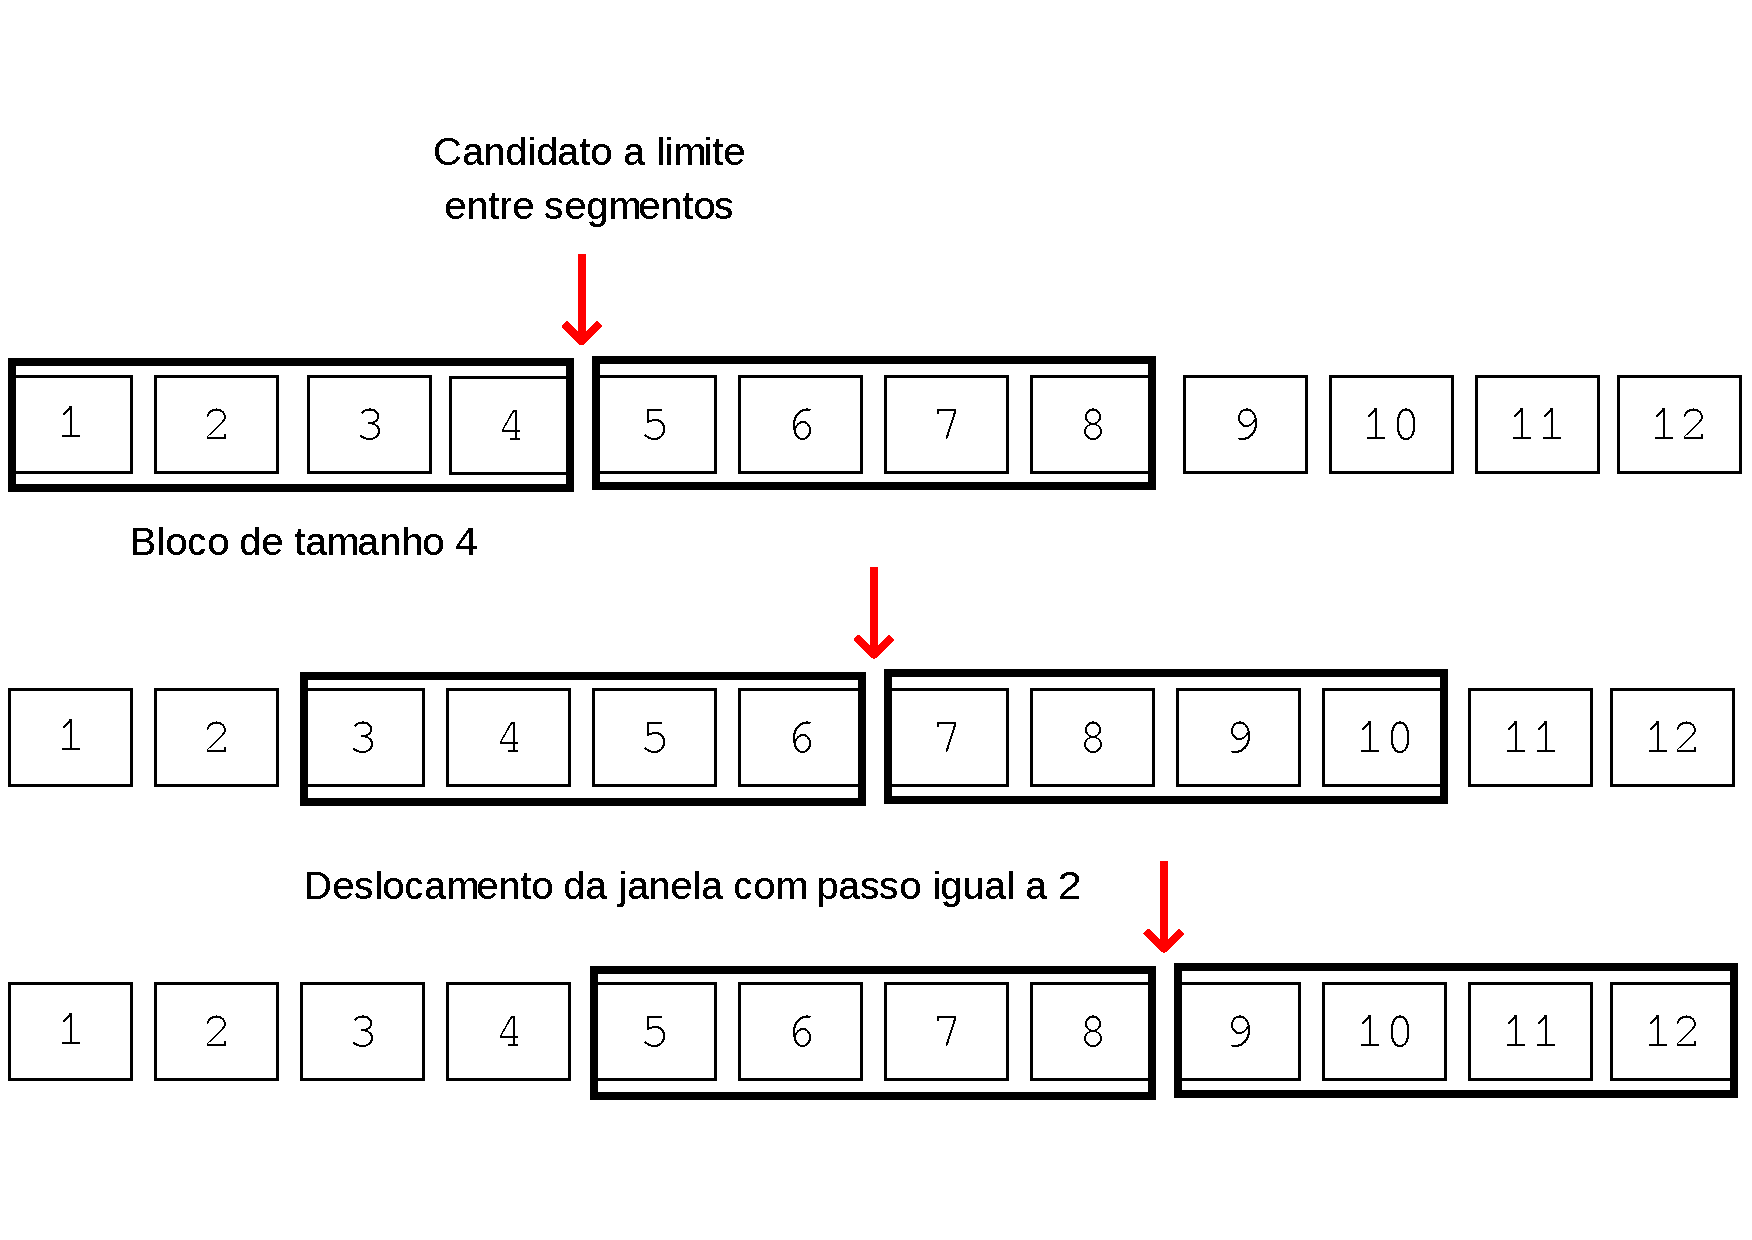
\includegraphics[trim={ 0 60 0 66 },clip,page=1,width=0.8\textwidth]{conteudo/capitulos/figs/janelas-deslizantes.pdf}

	\caption{Processo de deslocamento da janela deslizante. Os quadrados numerados representam as sentenças e os retângulos representam os blocos de texto a serem comparados. O deslocamento movimenta o candidato a limite e por consequência os blocos que o antecede e sucede.}
	\label{fig:TT-slidingwindow}
\end{figure}


Em seguida, os blocos de texto são representados por vetores que contém as frequências de suas palavras.  Diferente da proposta de Kozima, o \textit{TextTiling} utiliza cosseno (Equação~\ref{equ:cosine}) como medida para a similaridade entre os blocos adjacentes. Um limite ou transição entre segmentos é identificado sempre que a similaridade entre as unidades que antecedem e precedem o ponto candidato cai abaixo de um limiar, indicando uma diminuição da similaridade entre os blocos adjacentes. Ou seja, identifica-se uma transição entre segmentos pelos vales na curva de dissimilaridades. Para cada final de sentença representada por $c_i$ atribui-se uma profundidade dada por $(c_{i-1}-c_{i}) + (c_{i+1}-c_{i})$ e será um limite entre segmentos caso a profundidade exceda $\overline{s} - \sigma$, onde $\overline{s}$ é a média da profundidade de todos os vales do documento e $\sigma$, o desvio padrão. Na Figura~\ref{fig:curvasimilaridade} é ilustrado a curva de dissimilaridade entre os blocos adjacentes.  

   
\begin{figure}[h!]
\center
	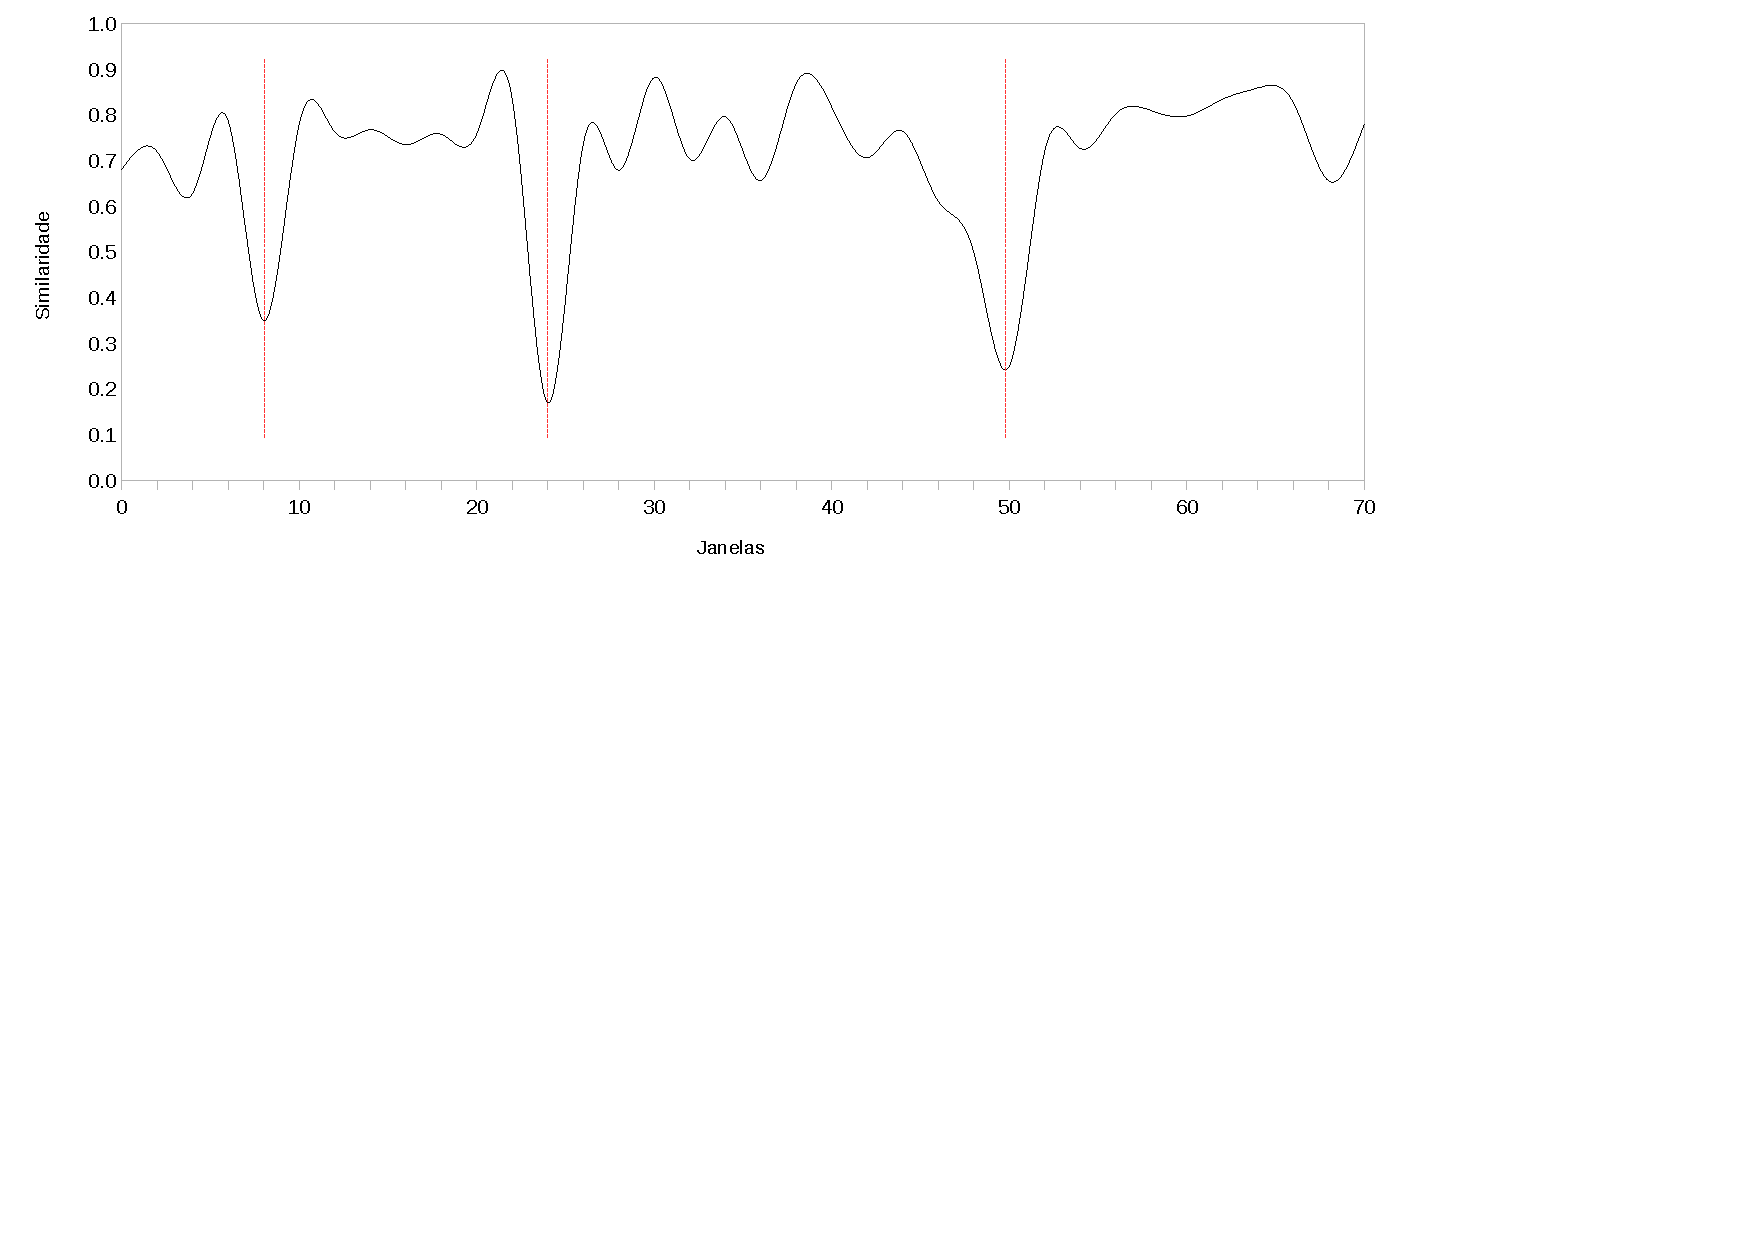
\includegraphics[trim={ 10 320 180 0 },clip,page=1,width=\textwidth]{conteudo/capitulos/figs/curva-similaridade.pdf}

	\caption{Curva de dissimilaridades entre blocos de texto adjacentes. As linhas pontilhadas representam diminuições de similaridade que indicam limites entre segmentos.}
	\label{fig:curvasimilaridade}
\end{figure}

% --> fazer um gráfico-rascunho e usar bolinhas para indicar os limites e usar 1 vale para demostrar o cálculo do depth score.


O TextTiling apresenta como vantagens a facilidade de implementação, 
% e baixa complexidade computacional, 
o que favorece o desenvolvimento de trabalhos similares 
~\cite{Naili2016,bokaei2015a,CHAIBI2014,Kern2009,Galley2003}, 
e sua utilização como \textit{base line} em outros trabalhos~\cite{Cardoso2017,Dias2007}. Por outro lado, algoritmos mais complexos, como os baseados em matrizes de similaridade, apresentam acurácia relativamente superior como apresentado em~\cite{Choi2000a, Kern2009, misra2009a}.


% ==========  C99  ==========

Outro algoritmo frequentemente referenciado na literatura é o C99~\cite{Choi2000a} o qual é baseado em uma matriz de \textit{ranking} das similaridades. A utilização de da coesão léxica pode não ser confiável para segmentos pequenos nessa abordagem, pois a ocorrência adicional de uma palavra pode causar certo impacto e alterar o cálculo da similaridade. Além disso, o estilo da escrita normalmente não é constante em todo o texto. Por exemplo, textos iniciais dedicados a introdução costumam apresentar menor coesão do que trechos dedicados a um tópico específico. Portanto, comparar a similaridade entre trechos de diferentes regiões não é apropriado. Devido a isso, as similaridades não podem ser comparadas em valores absolutos. Contorna-se esse problema fazendo uso de matrizes de similaridade para encontrar os segmentos de texto. Para isso, o \textit{C99} constrói uma matriz que contém as similaridades de todas as unidades de informação (normalmente sentenças ou parágrafos). 

%%%%%% 
%%%%%% 

Na Figura~\ref{fig:matrix-similarity} é mostrado um exemplo de uma matriz de similaridade onde a intensidade do ponto($i,j$) representa a similaridade entre as sentenças $i$ e $j$. Observa-se que a matriz é simétrica, assim cada ponto na linha diagonal representa a similaridade quando $i = j$ (ou seja, com a mesma sentença) e revela quadrados com maior concentração de pontos ao longo da diagonal. A concentração de pontos ao longo da diagonal indica porções de texto com maior coesão léxica.


  \begin{figure}[!h]
	  \centering
	  % 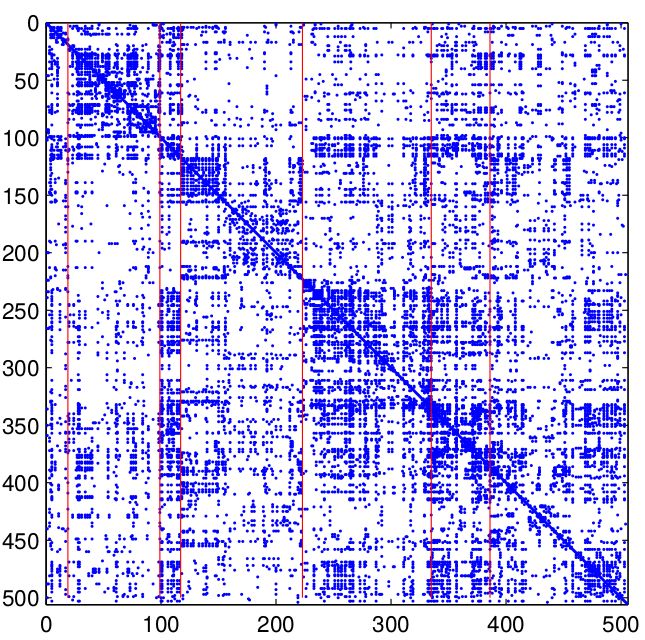
\includegraphics[width=0.6\textwidth]{conteudo/capitulos/figs/c99-ranking-matrix.png}
	  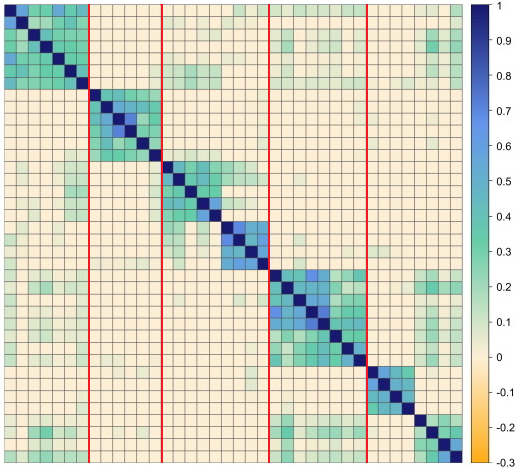
\includegraphics[width=0.6\textwidth]{conteudo/capitulos/figs/similarity-matrix-l.png}

	  % 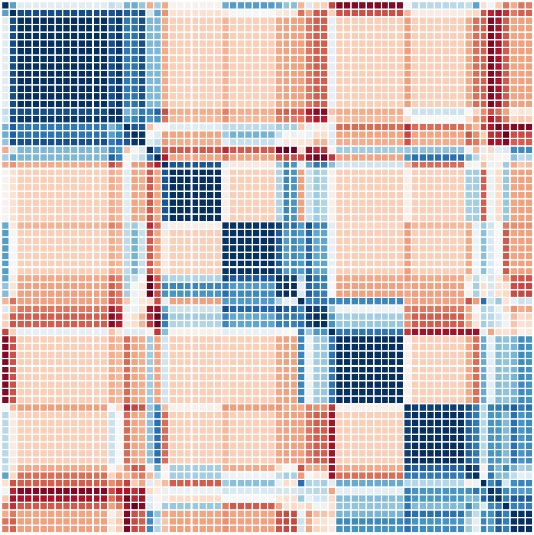
\includegraphics[width=0.6\textwidth]{conteudo/capitulos/figs/lda-sim-matrix.png}
	  \caption{\textit{DotPlot} da similaridade entre sentenças onde as linha verticais representam segmentos reais~\cite{Eis2008}.}
	  \label{fig:matrix-similarity}
  \end{figure}



%%%%%%%%%%%%%%%%%%%%%%%
% - Falar do esquema de ranking;
% - Imagem com os passos e máscara 3x3;
%%%%%%%%%%%%%%%%%%%%%%%

Em seguida, cada valor na matriz de similaridade é substituído por seu \textit{ranking} local. Para cada elemento da matriz, seu \textit{ranking} será o número de elementos vizinhos com valor de similaridade menor que o seu. Assim, para cada elemento determina-se uma região quadrada de tamanho $l$ em que o elemento em questão será comparado com $l \times l - 1$ elementos vizinhos.
% 
% 
Na Figura~\ref{fig:exemplomatrixrank} é destacado um quadro 3~x~3 de uma matriz. Tomando como exemplo o elemento com valor $0,5$, a mesma posição na matriz de \textit{rankings} terá o valor $4$, pois esse é o número de vizinhos com valores inferiores a $0,5$ dentro do quadro analisado na matriz de similaridades. Da mesma forma, 
% na Figura~\ref{fig:b} 
para o valor $0,2$ a matriz de \textit{rankings} conterá o valor $1$ na mesma posição. Após a construção da matriz de ranking obtêm-se um maior contraste entre os pontos, o que facilita a detecção de limites quando a queda de similaridade entre sentenças é mais sutil.

\begin{figure}[!h]
	\centering     %%% not \center

%	\subfigure[Passo 1]{
%		\label{fig:a}
		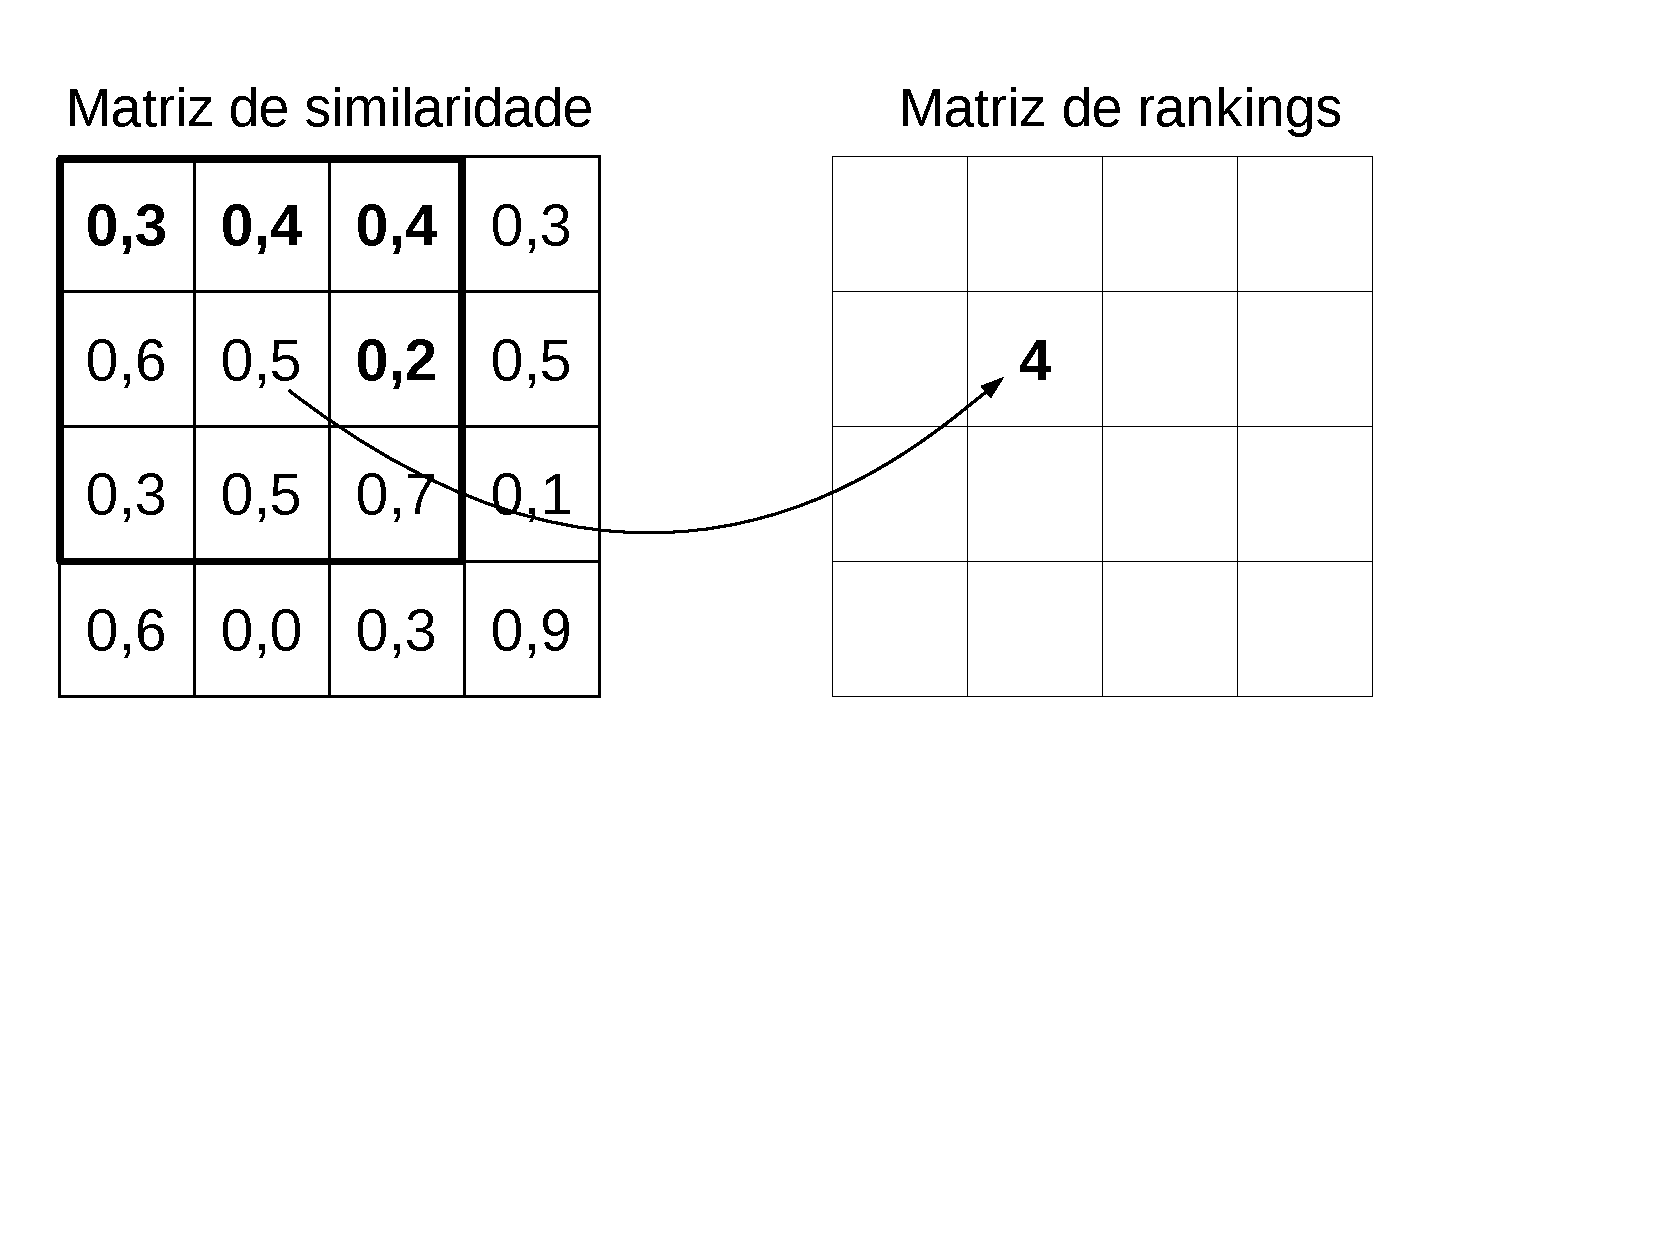
\includegraphics[trim={ 10 250 80 40 },clip,page=1,width=60mm]{conteudo/capitulos/figs/c99-matrizes.pdf}
%\\
%	}	
%	\subfigure[Passo 2]{
%		\label{fig:b}
		\includegraphics[trim={ 10 250 80 40 },clip,page=2,width=60mm]{conteudo/capitulos/figs/c99-matrizes.pdf}
		% 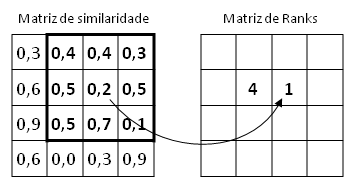
\includegraphics[width=60mm]{conteudo/capitulos/figs/exemplo-matrix-rank-B.png}
%	}
	\caption{Exemplo de construção de uma matriz de rankings.%~\cite{Choi2000}.
	}
	\label{fig:exemplomatrixrank}
\end{figure}
% -< Colocar uma explicação mais detalhada para esses passos


Finalmente, com base na matriz de \textit{ranking}, o C99 utiliza um método de \textit{clustering} baseado no algoritmo \textit{DotPloting}~\cite{Reynar1998} que usa regiões com maior densidade em uma matriz de similaridades para determinar como os segmentos estão distribuídos.  
% 
Um segmento é definido por duas sentenças $c_i$ e $c_j$ (respectivamente a primeira e última sentença do segmento) que representam uma região quadrada ao longo da diagonal da matriz. 
% 
Seja $S = \{s1,...,s_h\}$ a lista de $h$ segmentos,  $som_b$ a somatória dos valores dos \textit{rankings} de um segmento $s \in S$ e $a_s$ a sua área. Então, a densidade é computada por: 
% 
Calcula-se a densidade dessa região como mostrado na Equação~\ref{equ:densidade-c99}. 



\begin{equation}
Den = \frac{\sum_{s=1}^h som_s}{\sum_{s=1}^m a_b}
\label{equ:densidade-c99}
\end{equation}


O processo inicia com um único segmento formado por todas as sentenças do documento e o divide recursivamente em $m$ segmentos. Cada passo divide $B$ no ponto ($i,j$) que maximiza $Den$~(Equação \ref{equ:densidade-c99}). O processo se repte até atingir o número de segmentos desejados ou um limiar de similaridade.

% ===



% \textbf{Abordagens probabilísticas}

% ==========  TextSeg Utiyama and Isahara  ==========


Desenvolveu-se também abordagens probabilísticas para segmentação textual, por exemplo, o método proposto por~\cite{Utiyama2001} encontra a segmentação por meio de um modelo estatístico. Dado um texto representado por um conjunto de palavras 
$W = \{w_1, w_2, \dots, w_n\}$ e um conjunto de segmentos $S = \{s_1, s_2, \dots, s_h\}$ que segmenta $W$, a probabilidade da segmentação S é dada por:

\begin{equation}
	P(S|W) = \frac{P(W|S)P(S)}{P(W)}
\end{equation}

Com isso, é possível encontrar a sequência de segmentos mais provável $\hat{S} = arg max_S~P(W|S) P(S)$. Nesse trabalho assume-se que os segmentos são estaticamente independentes entre si e as palavras nos segmentos são independentes dado o segmento que as contém. Essa simplificação permite decompor o termo $P(W|S)$ em um produtório de ocorrência de das palavras dado um segmento,  

\begin{equation}
	P(W|S) = \prod_{i=1}^m \prod_{j=1}^n P(w_j^i|S_i) ~ ,
\end{equation}


\noindent
onde $P(w_j^i|S_i)$ é a probabilidade da j-ésima palavra ocorrer no segmento $S_i$ a qual é definida na Equação~\ref{equ:Utiyama2}. Seja $f_i(w_j)$ a frequência da j-ésima palavra no i-ésimo segmento, $n_i$ é o número de palavras em $S_i$ e $k$ é o número de palavas diferentes em $W$. Calcula-se: 

\begin{equation}
	P(w_j^i|S_i) = \frac{f_i(w_j) + 1}{n_i + k}
	\label{equ:Utiyama2}
\end{equation}

A suposição de independência entre segmentos e as palavras neles contidas, são é verificada no mundo real. Para segmentos muito pequenos a estimativa das probabilidades das palavras pode ser afetada. Além disso, o modelo não leva em conta a importância relativa das palavras~\cite{Malioutov:2006a}.

 


% ===

% ==========  BayesSeg  ==========

Os métodos baseados em coesão léxica que utilizam métricas como cosseno quantificam a similaridade entre sentenças baseando-se apenas na frequência das palavras, Essa abordagem, ignora certas características do texto que podem dar pistas sobre a estrutura do texto. Por exemplo, frases como ``\textit{Prosseguindo}'', ``\textit{Dando continuidade}'', ``\textit{Ao final da reunião}'' podem ajudar a detectar o inicio ou final de segmento. A fim de aproveitar esses indicadores, pode-se usar um framework bayesiano que permite incorporar fontes externas ao modelo. O método \textit{BayesSeg}~\cite{Eis2008} aborda a coesão léxica em um contexto bayesiano onde as palavas de um segmento surgem de um modelo de linguagem multinomial o qual é associado a um assunto. 
%
Essa abordagem é similar à métodos probabilísticos de extração de tópicos como o Latent Dirichlet Allocation (LDA)~\cite{Blei2003}, com a diferença que ao invés de atribuir tópicos ocultos a cada palavra, esses são usados para segmentar o documento. Nesse sentido, detecta-se um limite entre sentenças quando a distribuição de tópicos entre elas for diferente. O \textit{BayesSeg} baseia-se na ideia que alguns termos são usados em tópicos específicos enquanto outros são neutros em relação aos tópicos do documento e são usados para expressar uma estrutura do documento, ou seja, as frases-pista vem de um único modelo generativo. A fim de refletir essa ideia, o modelo é adaptado para influenciar a probabilidade da sentença de ser uma final ou início de segmento conforme a presença de frases pista.

% ===


% ==========  MinCut  ==========

% file:///ext4Data/UFSCar/Dissertação-2018/referencias/Minimum Cut Model for Spoken Lecture Segmentation - article.pdf




O \textit{MinCutSeg} ~\cite{Malioutov:2006a} aborda a segmentação textual como um problema de particionamento de grafo, em que cada nó representa um sentença e os pesos das arestas representam a similaridade entre duas sentenças (Figura~\ref{fig:representacao-texto-grafo}). Nessa abordagem, a segmentação textual corresponde ao particionamento do grafo que representa o texto.


  \begin{figure}[!h]
	  \centering
	  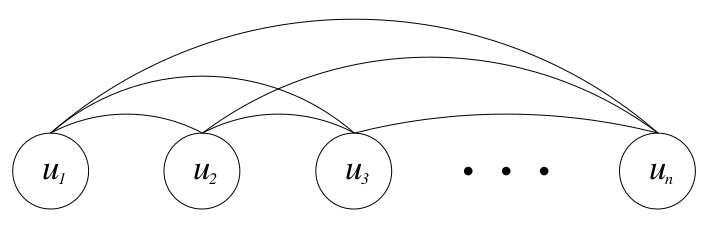
\includegraphics[width=0.6\textwidth]{conteudo/capitulos/figs/graph-representation-of-text.png}
	  \caption{Representação de texto baseada em grafo~\cite{Malioutov:2006a}}
	  \label{fig:representacao-texto-grafo}
  \end{figure}


Essa abordagem é inspirada no trabalho de~\cite{Shi2000} que propõe um critério para particionamento de grafos chamado \textit{normalized-cut criterion} inicialmente desenvolvido para segmentação de imagens estáticas a qual foi aproveita a restrição de linearidade dos textos para segmentação textual.

Seja $G = {V,E}$ um grafo ponderado, unidimensional em que $V$ é o conjunto de vértices que correspondem às sentenças e $E$ é o conjunto de arestas que correspondem as similaridades entre as sentenças. Seja $sim(u, v)$ o valor de similaridade entre o par de vértices $u$ e $v$. O \textit{MinCutSeg} visa particionar $G$ em dois grafos disjuntos $A$ e $B$ de modo a minimizar o corte definido pela somatória das arestas que ligam $u \in A$ à $v \in B$(Equação~\ref{equ:corte-grafo}):

\begin{equation} 
	corte(A,B) = \sum_{u \in A,v \in B} sim(u, v) 
	\label{equ:corte-grafo}
\end{equation}



Além de maximizar a diferença entre as partições $A$ e $B$, é necessário que essas seja homogenias em relação a similaridade de suas sentenças, conforme requerimento definido por~\cite{Shi2000} em que o valor do corte deve ser normalizado pelo volume das partições dado por:

\begin{equation}
	vol(A) = \sum_{u \in A, v \in V} sim(u, v)
\end{equation}


Em seguida, define-se o critério de corte normalizado (NCorte) como o resultado da normalização do corte pelo volume, conforme mostrado na Equação~\ref{equ:NCorte}.

\begin{equation}
	NCorte(A,B) = \frac{corte(A,B)}{vol(A} + \frac{corte(A,B)}{vol(B)}
	\label{equ:NCorte}
\end{equation}


Uma vez que um texto normalmente é dividido em mais que dois segmentos, é necessário extender o modelo para atender a essa necessidade. Seja $A_1 \dots A_k$ uma partição e $V - A_k$ a diferença entre o grafo $V$ e a partição $k$. O critério para múltiplos cortes normalizados é então estendido para: 

\begin{equation} 
	NCorte_k(V) = \frac{corte(A_1, V-A_1)}{vol(A_1)} + \dots + \frac{corte(A_k, V-A_k)}{vol(A_k)} 
	\label{equ:NCorte-k}
\end{equation}


A decomposição do modelo em uma somatória de termos individuais permite empregar técnicas de programação dinâmica para o problema de cortes multidirecionais em grafos. Mais detalhes da formulação dessa solução estão disponíveis em~\cite{Malioutov:2006a}.

Embora o problema minimizar cortes normalizados em grafos seja um problema do tipo NP-Completo\footnote{NP-Completo configura um tipo de problema para o qual não se conhece uma solução determinística que possa ser computada em tempo polinomial. Papadimitriou provou que o problema de corte mínimo em grafos está incluso nessa categoria.}, no contexto de segmentação textual esse problema é restrito a manter a linearidade dos vértices. A segmentação linear em um grafo implica que todos os vértices entre as extremidades esquerda e direitas de uma partição pertencem à essa partição, consequentemente o espaço de soluções possíveis é reduzido o que permite a execução do algoritmo em tempo polinomial.  

% ===
















 


% -- Medidas
\subsection{Medidas de Avaliação em Segmentação Textual}
\label{subsec:medidas-segmentacao}

% 


As medidas de avaliação tradicionais como precisão e revocação são permitem medir o desempenho de modelos de Recuperação de Informação e Aprendizado de Máquina por meio da comparação dos valores produzidos pelo modelo com os valores observados em uma referência. 
%	Avaliações baseadas em hits 
Usa-se uma tabela, chamada matriz de confusão, para visualizar o desempenho de um algoritmo. Na Tabela~\ref{tab:matrizconfusao} é apresentada uma matriz de confusão para duas classes (Positivo e Negativo). 

\begin{table}[!h]
\centering

\begin{tabular}{|c|c|c|}
  \hline
				& Predição Positiva        & Predição Negativa        \\ \hline
  Positivo real & VP (Verdadeiro Positivo) & FN (Falso Negativo)      \\ \hline
  Negativo real & FP (Falso Positivo)      & VN (Verdadeiro Negativo) \\ \hline

\end{tabular}

\caption{Matriz de confusão.}
\label{tab:matrizconfusao}

\end{table}


%
% Falso Positivo 
% Falso Negativo 
% Verdadeiro Positivo 
% O Verdadeiro Negativo, que não existe 
%%% 
No contexto de segmentação textual, um falso positivo é um limite identificado pelo algoritmo que não corresponde a nenhum limite na segmentação de referência, ou seja, o algoritmo indicou que em determinado ponto há uma quebra de segmento, mas na segmentação de referência, no mesmo ponto, não há. De maneira semelhante, um falso negativo é quando o algoritmo não identifica um limite existente na segmentação de referência, ou seja, em determinado ponto há, na segmentação de referência, um limite entre segmentos, contudo, o algoritmo não o identificou.  Um verdadeiro positivo é um ponto no texto indicado pelo algoritmo e pela segmentação de referência como uma quebra de segmentos, ou seja, o algoritmo e a referência concordam que em determinado ponto há uma transição de assunto.  Na avaliação de segmentadores, não há o conceito de verdadeiro negativo. Este seria um ponto no texto indicado pelo algoritmo e pela segmentação de referência onde não há uma quebra de segmentos. Uma vez que os algoritmos apenas indicam onde há um limite, essa medida não é necessária. % Não há ou não e necessário?


% 
% Precisão 
%%%
Nesse sentido, a precisão indica a proporção de limites corretamente identificados pelo algoritmo, ou seja, correspondem a um limite real na segmentação de referência. 
Porém, não diz nada sobre quantos limites reais existem. 
É calculada dividindo-se o número de limites identificados automaticamente pelo número de candidatos a limite (Equação~\ref{equ:precisao}).
 
 \begin{equation}
	 Precis\tilde{a}o = \frac{VP}{VP+FP}
	 \label{equ:precisao}
 \end{equation}

%
% Revocação 
%%%
 A revocação, é a proporção de limites verdadeiros que foram identificados pelo algoritmo. Porém não diz nada sobre quantos limites foram identificados incorretamente. É calculada dividindo-se o número de limites identificados automaticamente pelo número limites verdadeiros (Equação~\ref{equ:revocacao}).
 
 \begin{equation}
	 Revoca\c{c}\tilde{a}o = \frac{VP}{VP+FN}
	 \label{equ:revocacao}
 \end{equation}

 Existe uma relação inversa entre precisão e revocação. Conforme o algoritmo aponta mais segmentos no texto, este tende a melhorar a revocação e ao mesmo tempo, reduzir a precisão. Esse problema de avaliação pode ser contornado utilizado a medida $F^1$ que é a média harmônica entre precisão e revocação onde ambas tem o mesmo peso (Equação~\ref{equ:f1}). 

 \begin{equation}
	 F^1 = \frac{2 \times Precis\tilde{a}o \times Revoca\c{c}\tilde{a}o}
		        {Precis\tilde{a}o + Revoca\c{c}\tilde{a}o}
	 \label{equ:f1}
 \end{equation}



%-> Precisão é a fração de instâncias recuperadas que são relevantes, 
%-> Revocação é a fração de instâncias relevantes que são recuperadas.
%-> https://pt.wikipedia.org/wiki/Precis%C3%A3o_e_revoca%C3%A7%C3%A3o





























As medidas de avaliação tradicionais como precisão e revocação permitem medir o desempenho de modelos de Recuperação de Informação e Aprendizado de Máquina por meio da comparação dos valores produzidos pelo modelo com os valores observados em uma referência. 
%	Avaliações baseadas em hits 
Usa-se uma tabela, chamada matriz de confusão, para visualizar o desempenho de um algoritmo. Na Tabela~\ref{tab:matrizconfusao} é apresentada uma matriz de confusão para duas classes (Positivo e Negativo). 


\begin{table}[!h]
\centering

\begin{tabular}{|c|c|c|}
  \hline
				& Predição Positiva        & Predição Negativa        \\ \hline
  Positivo real & VP (Verdadeiro Positivo) & FN (Falso Negativo)      \\ \hline
  Negativo real & FP (Falso Positivo)      & VN (Verdadeiro Negativo) \\ \hline

\end{tabular}

\caption{Matriz de confusão.}
\label{tab:matrizconfusao}

\end{table}


% -> Falso Positivo % Falso Negativo % Verdadeiro Positivo % O Verdadeiro Negativo, que não existe 

No contexto de segmentação textual, um falso positivo é um limite identificado pelo algoritmo que não corresponde a nenhum limite na segmentação de referência, ou seja, o algoritmo indicou que em determinado ponto há uma quebra de segmento, mas na segmentação de referência, não há quebra no mesmo ponto. De maneira semelhante, um falso negativo é quando o algoritmo não identifica um limite existente na segmentação de referência, ou seja, em determinado ponto há, na segmentação de referência, um limite entre segmentos, contudo, o algoritmo não o identificou.  Um verdadeiro positivo é um ponto no texto indicado pelo algoritmo e pela segmentação de referência como uma quebra de segmentos, ou seja, o algoritmo e a referência concordam que em determinado ponto há uma transição de assunto.  Na avaliação de segmentadores, não há o conceito de verdadeiro negativo. Este seria um ponto no texto indicado pelo algoritmo e pela segmentação de referência onde não há uma quebra de segmentos. Uma vez que os algoritmos apenas indicam onde há um limite, essa medida não é necessária. % Não há ou não e necessário?


% -> Precisão 
Nesse sentido, a precisão indica a proporção de limites corretamente identificados pelo algoritmo, ou seja, correspondem a um limite real na segmentação de referência. 
Porém, não diz nada sobre quantos limites reais existem. 
É calculada dividindo-se o número de limites identificados automaticamente pelo número de candidatos a limite (Equação~\ref{equ:precisao}).
 
 \begin{equation}
	 Precis\tilde{a}o_{seg} = \frac{VP}{VP+FP}
	 \label{equ:precisao}
 \end{equation}


% -> Revocação 

 A revocação, é a proporção de limites verdadeiros que foram identificados pelo algoritmo. Porém não diz nada sobre quantos limites foram identificados incorretamente. É calculada dividindo-se o número de limites identificados automaticamente pelo número limites verdadeiros (Equação~\ref{equ:revocacao}).
 
 \begin{equation}
	 Revoca\c{c}\tilde{a}o_{seg} = \frac{VP}{VP+FN}
	 \label{equ:revocacao}
 \end{equation}

 Existe uma relação inversa entre precisão e revocação. Conforme o algoritmo aponta mais segmentos no texto, este tende a melhorar a revocação e ao mesmo tempo, reduzir a precisão. Esse problema de avaliação pode ser contornado utilizado a medida $F^1$ que é a média harmônica entre precisão e revocação onde ambas tem o mesmo peso (Equação~\ref{equ:f1}). 

 \begin{equation}
	 {F^1}_{seg} = \frac{2 \times Precis\tilde{a}o \times Revoca\c{c}\tilde{a}o}
		        {Precis\tilde{a}o + Revoca\c{c}\tilde{a}o}
	 \label{equ:f1}
 \end{equation}



%-> Precisão é a fração de instâncias recuperadas que são relevantes, 
%-> Revocação é a fração de instâncias relevantes que são recuperadas.
%-> https://pt.wikipedia.org/wiki/Precis%C3%A3o_e_revoca%C3%A7%C3%A3o

% =============================================================


%  Medidas de avaliação tradicionais 
As medidas de avaliação tradicionais, precisão e revocação, podem não ser confiáveis, por não considerarem a distância entre os limites, mas penalizam o algoritmo sempre que um limite que não coincide perfeitamente com a referência. Essas medidas podem ser mais adequadas quando necessita-se de segmentações com maior exatidão. Em outras palavras, computam apenas os erros do algoritmo quando se detecta falsos positivos ou falsos negativos, o que nesse contexto de segmentação textual pode não ser suficiente, dado a subjetividade da tarefa. Além dessas medidas, que consideram apenas se um segmento foi perfeitamente definido conforme uma referência, pode-se também considerar a distância entre o segmento extraído automaticamente e o segmento de referência~\cite{Kern2009}. Chama-se \textit{near misses} o caso em que um limite identificado automaticamente não coincide exatamente com a referência, mas é necessário considerar a proximidade entre eles.

%  Medidas que consideram a distancia entre os segmentos 
Na Figura~\ref{fig:exemplosegmentacaozoom} é apresentado um exemplo com duas segmentações extraídas automaticamente e uma referência. Em ambos os casos não há nenhum verdadeiro positivo, o que implica em zero para os valores de precisão, acurácia, e revocação, embora o resultado do algoritmo A possa ser considerado superior ao primeiro se levado em conta a proximidade dos limites.
% Para não confundir hipótese com algoritmo, escrever: "A hipótese A, produzida pelo algoritmo A e a hipótese B, produzida pelo algoritmo B".
% Ou trocar hipótese por resultado do algoritmo A, B

  \begin{figure}[!h]

	\centering
	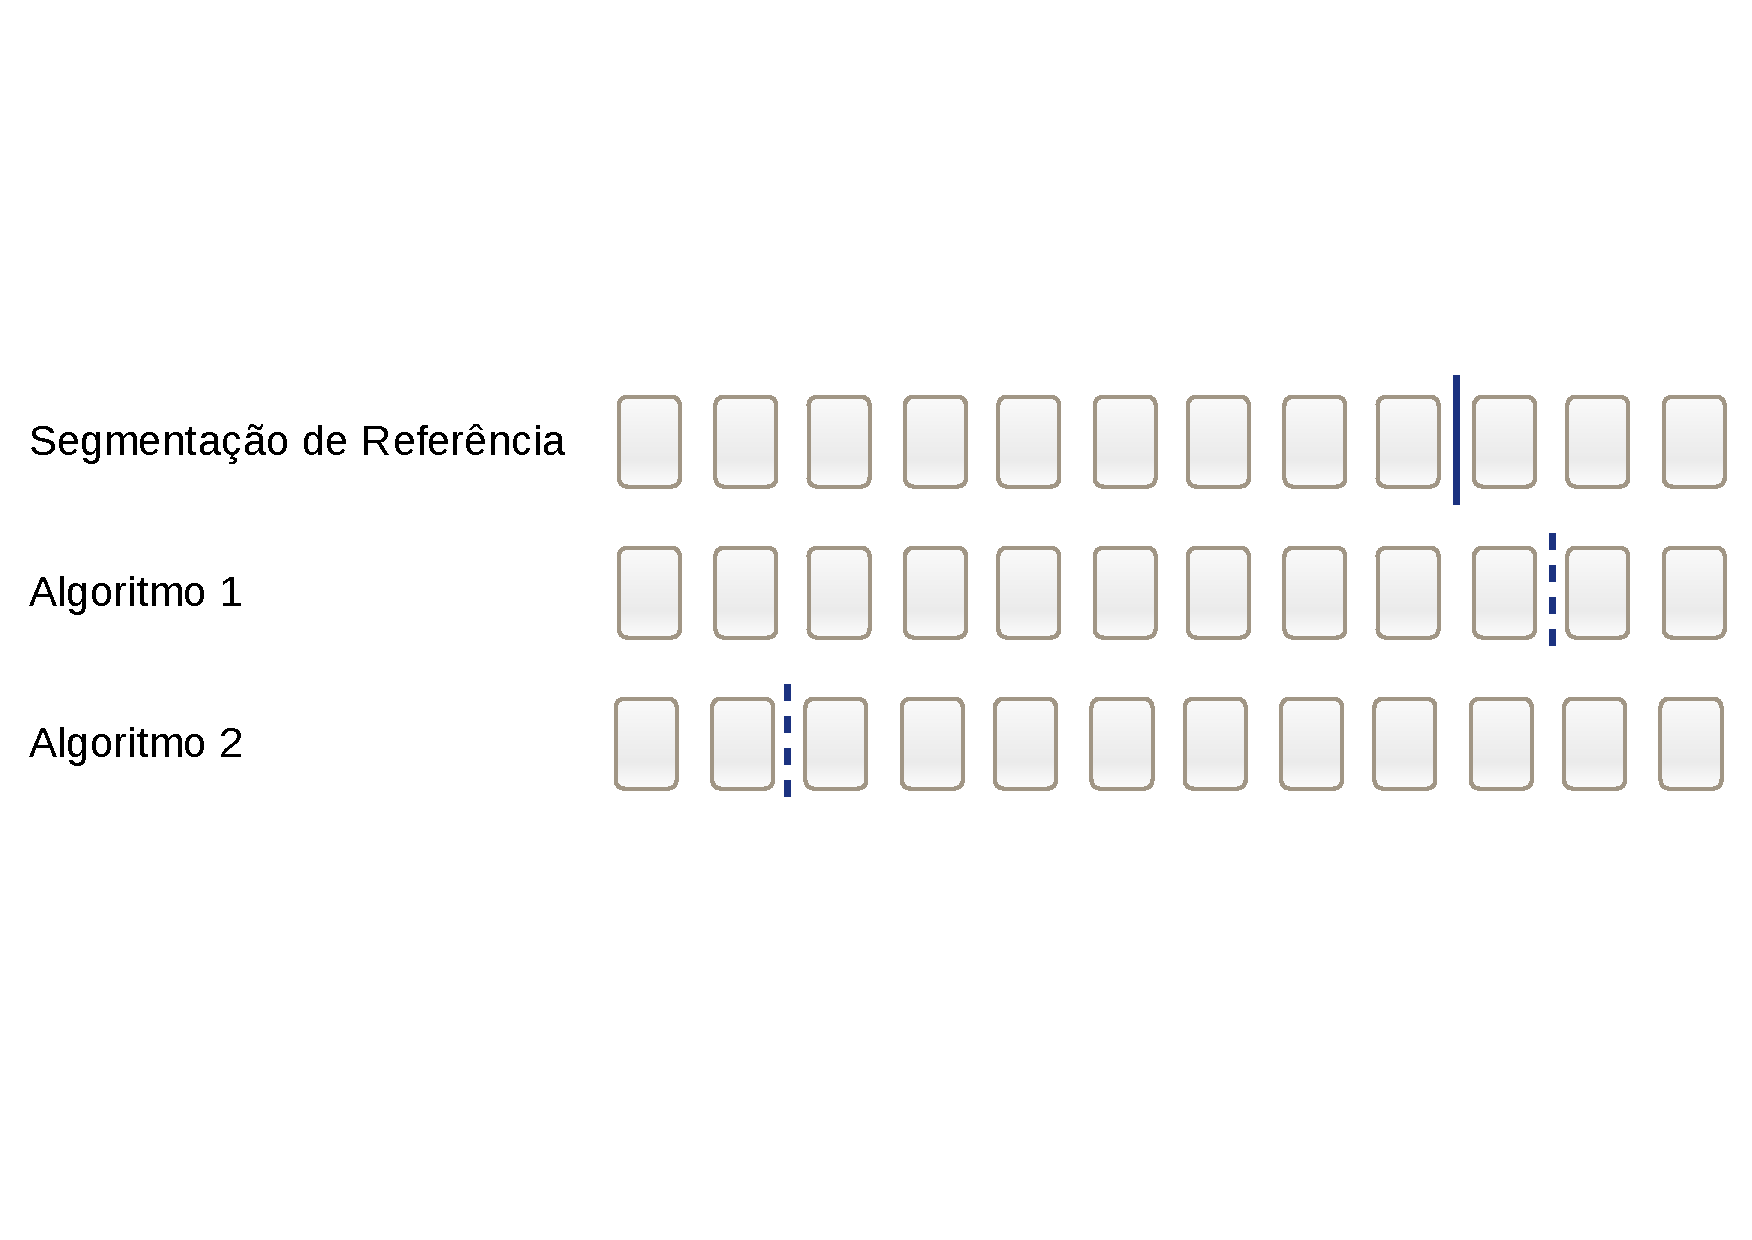
\includegraphics[trim={ 0 180 0 180 },clip,page=1,width=0.7\textwidth]{conteudo/capitulos/figs/near-missing.pdf}
	\caption{Exemplos de \textit{near missing} e falso positivo puro. Os blocos indicam uma unidade de informação e as linha verticais representam uma transição de assunto. }
	\label{fig:exemplosegmentacaozoom}

  \end{figure}
  


% === PK ===

Considerando o conceito de \textit{near misses}, algumas medidas de avaliação foram propostas. Proposta por~\cite{Beeferman1999}, P$_k$ atribui valores parciais a \textit{near misses}, ou seja, limites sempre receberão um peso proporcional à sua proximidade, desde que dentro de um janela de tamanho~$k$.  Para isso, esse método move uma janela de tamanho $k$ ao longo do texto. A cada passo verifica, na referência e no algoritmo, se as extremidades (a primeira e última sentença) da janela estão ou não dentro do mesmo segmento, então, penaliza o algoritmo caso este não concorde com a referência. Ou seja, dado dois termos de distância $k$, $P_k$ verifica se o algoritmo coloca os termos no mesmo segmento ou em segmentos distintos e o penaliza caso não concorde com a referência. Dadas uma segmentação de referência $ref$ e uma segmentação automática $hyp$, ambas com $N$ sentenças, P$_k$ é computada como:


\begin{equation}
P_k(ref,hyp) = \frac{1}{N - k}
\sum_{i=1}^{N-k } 
(
\delta_{ref}(i, i+k) ~
\bar{\oplus} ~
\delta_{hyp}(i, i+k) 
)
\label{equ:Pk}
\end{equation}


Onde $\delta_S(i,j)$ é a função indicadora que retorna 1 se as sentenças $c_i$ e $c_j$ estão no mesmo segmento e 0 caso contrário, $\bar{\oplus}$ é o operador \texttt{XNOR} (ambos ou nenhum) que retorna 1 se ambos os argumentos forem diferentes. 
%
%
O valor de $k$ é calculado como a metade da média dos comprimentos dos segmentos reais. Como resultado, é retornada a dissimilaridade entre a segmentação calculada pela contagem de discrepâncias divida pela quantidade de segmentos analisados. Essa medida pode ser interpretada como a probabilidade de duas sentenças extraídas aleatoriamente pertencerem ao mesmo segmento.  




% === WindowDiff ===

\textit{WindowDiff}~\cite{Pevzner2002} é uma medida alternativa à P$_k$. De maneira semelhante, move uma janela pelo texto e penaliza o algoritmo sempre que o número de limites proposto pelo algoritmo não coincidir com o número de limites esperados para aquela janela. Ou seja, o algoritmo é penalizado quando não concordar com a segmentação de referência quanto ao número de segmentos na janela. Mais formalmente, para cada intervalo $k$, compara o número de segmentos obtidos pela referência $r_i$ com o obtido pelo algoritmo $a_i$ e penaliza o algoritmo se $r_i \neq a_i$. Na Equação~\ref{equ:windiff} é mostrada a definição de WindowDiff onde $b(i, i+k)$ representa o número de limites entre as sentenças $i$ e $i+k$ e $N$, o total de sentenças no texto.
% e $k = \frac{N}{2 \times n\'{u}mero\ de\ segmentos}$. 

\begin{equation}
	WindowDiff(ref,hyp) = \frac{1}{N-k}\sum_{i=1}^{N-k}(|b(ref_i - ref_{i+k}) - b(hyp_i - hyp_{i+k})| > 0)
	\label{equ:windiff}
\end{equation}


Assim, consegue manter a sensibilidade a \textit{near misses} e além disso, considerar o tamanho das janelas.  A fim de melhor equilibrar o peso dos falsos positivos em relação a \textit{near misses}, dobra-se a penalidade para falsos positivos, evitando-se a supervalorização dessa medida.  % OBS: Os problemas de Pk ficaram subentendidos aqui :/ 

As medidas \textit{WindowDiff} e P$_k$, consideram a quantidade e proximidade entre os limites, sendo mais tolerantes a pequenas imprecisões. Essa é uma característica desejável, visto que as segmentações de referência possuem diferenças consideráveis. \textit{WindowDiff} equilibra melhor os falsos positivos em relação a \textit{near misses}, ao passo que P$_k$ os penaliza com peso maior. Isso significa que segmentadores melhores avaliados em P$_k$ ajudam a selecionar as configurações que erram menos ao separar trechos de texto com o mesmo assunto, enquanto \textit{WindowDiff} é mais tolerante nesse aspecto.  De maneira geral, observa-se  melhores resultados de \textit{WindowDiff} quando os algoritmos aproximam a quantidade de segmentos automáticos da quantidade de segmentos da referência. Por outro lado, P$_k$ avalia melhor as configurações que retornam menos segmentos. Contudo, não é possível definir um valor adequado, uma vez que os segmentadores humanos frequentemente apontam segmentações diferentes.






% --> encerramento da seção de segmentação.
Ao final do processo de segmentação, são produzidos fragmentos de documentos, aqui chamados de subdocumentos. Esses subdocumentos contém um texto, assim como no documento original, em um estágio de processamento inicial, pois ainda não estão estruturados. Ocorre que as técnicas de aprendizado de máquina exigem uma representação estruturada dos textos conforme será visto na Seção~\ref{section:RepTextos}.





